\documentclass[a4paper,10pt]{article}
\usepackage[utf8]{inputenc}
\usepackage[brazilian]{babel}
\usepackage[justification=centering]{caption}
\usepackage[hmargin=2cm,vmargin=3.5cm,bmargin=2cm]{geometry}
\usepackage[table,xcdraw]{xcolor}
\usepackage{indentfirst}
\usepackage{amsmath}
\usepackage{graphicx}
\usepackage{makeidx}
\usepackage{tocbibind}
 
 \begin{document}	
	\begin{titlepage}
		\begin{center}
		{\large UNIVERSIDADE ESTADUAL DE MARINGÁ}\\[0.2cm]
		{\large CENTRO DE CIÊNCIAS EXATAS}\\[0.2cm]
		{\large DEPARTAMENTO DE FÍSICA}\\[0.2cm]
		{\large LABORATÓRIO DE FÍSICA MODERNA}\\[7.0cm]
		{\bf \huge Interferômetro}\\[7.0cm]
		\end{center}
	{\large Adão Murillo dos Santos \hfill RA:100126}\\[0.7cm]
	{\large João Marcos Fávaro Lopes \hfill RA:98327}\\[0.7cm]
	{\large Lucas Maquedano da Silva \hfill RA:98901}\\[0.7cm]
	{\large Pedro Haerter Pinto \hfill RA:100852}\\[0.7cm]
	{\large TURMA:32 \hfill Professor: Nelson Guilherme Castelli
	Astrath}
	
	\vfill
		\begin{center}
		{\large Maringá,2018}
		\end{center}
	\end{titlepage}

	\tableofcontents
	\section{Introdução}
Interferência é um fenômeno que ocorre quando duas ou mais ondas sobrepostas se encontram fora de fase, gerando interferências construtivas e destrutivas conforme a interação entre as ondas, sendo a luz uma onda eletro magnética o fenômeno também se aplica a ela, como foi observado no experimento de fenda dupla de Young, as ondas de luz emitidas a partir das fendas se sobrepõem e criam faixas escuras e claras sendo estas os mínimos e máximos de intensidade luminosa gerados pela interferência. Michelson montou o seu interferômetro, aparato que foi utilizado no experimento contido neste relatório, a fim de mostrar a influência do "éter luminoso"(suposto meio necessário para a propagação da luz) sobre a velocidade da luz, o experimento mostrou a não existência do éter. 
No presente relatório, o interferômetro de Michelson será utilizado para determinar o comprimento de onda de um lazer.

	\section{Desenvolvimento Teórico}
\subsection{Razão Carga Massa}
A força magnética atuante em uma partícula eletricamente carregada de carga {\it q} num campo magnético {\it B} é dado pela equação
\begin{equation}
F_m = qv \times B
\end{equation}
Onde {\it v} é a velocidade da partícula. Para o caso em que a velocidade é perpendicular à direção do campo, a equação pode ser simplificada para a forma escalar
\begin{equation}
	F_m = evB
\end{equation}
Em que {\it e} é a carga elementar do elétron. Como os elétrons do feixe realizarão um movimento circular dentro do bulbo de vidro, estes estarão sujeitos a uma força centrípeta de forma
\begin{equation}
	F_c = \frac{mv^2}{r}
\end{equation}
Onde {\it m} é a massa do elétron,{\it v} sua velocidade e {\it r} o raio do movimento circular. Como a força centrípeta é a única força externa agindo sobre o elétron, é possível igualar as duas equações de modo que
\begin{equation}
	F_m = F_c
\end{equation}
\begin{equation}
	evB = \frac{mv^2}{r}
\end{equation}
Como o objetivo é determinar a relação carga/massa, deve-se isolar esse quociente de modo a se obter seu valor em função dos demais valores
\begin{equation}
	\frac{e}{m}=\frac{v}{rB}
	\label{eq: em}
\end{equation}
A velocidade do elétron é determinada a partir da energia cinética dos elétrons sujeitos ao campo magnético, ou seja
\begin{equation}
	eV = \frac{1}{2}mv^2
\end{equation}
\begin{equation}
	\\ v = \left(\frac{2ev}{m}\right)^{\frac{1}{2}}
	\label{eq: v}
\end{equation}
O campo magnético produzido por um par de bobinas de Helmholtz é, nas proximidades do centro dado dado pela equação
 \begin{equation}
 	B = \frac{[N\mu _0]I}{a\left(\frac{5}{4}\right)^{\frac{3}{2}}}
	\label{B}
 \end{equation}
Substituindo \ref{eq: v} e \ref{B} na equação \ref{eq: em},
\begin{equation}
	\frac{e}{m}=\frac{v}{rB}=\frac{2V\left(\frac{5}{4}\right)^3a^2}{[N\mu _0 Ir]^2}
	\label{e/m}
\end{equation}
Onde $V$ é a energia potencial dos elétrons, $a$ o raio das bobinas de Helmholtz, $N$ o número de espiras em cada bobina de Helmholtz, $\mu _0$ a permeabilidade elétrica do meio, $I$ a corrente elétrica gerada nas bobinas e $r$ o raio de feixe de elétrons.

É possível determinar a relação carga/massa facilmente por este último resultado visto que é composto por constantes($N=130$ e $\mu _0 =4\pi 10^{-7}$) e valores que são ajustados nas fontes no decorrer do experimento.
\subsection{Desvios}
  \subsubsection{Desvio de Medidas Diretas}
  Para este experimento, tem-se como medidas diretas, o raio do feixe de elétrons formado dentro do tubo, sendo utilizada uma régua que a menor partição tem $1mm$ o erro associado é de $0,5mm$ ou $0,0005m$, e também a amperagem e voltagem utilizada nas bobinas de Helmholtz, sendo um multímetro digital, seu erro é $\pm 1$ a menor unidade.
  \subsubsection{Desvio de Medidas Indiretas}
  Para o cálculo da razão carga massa é utilizada a equação \ref{e/m}, mas substituindo $V$ e $r^2$ por $\lambda$ se obtém a igualdade \ref{eq1} e para o cálculo dos erros, é aplicado o logaritmo neperiano em ambos os lados da equação, tornando-se:
  \begin{equation}
      ln\left(\frac{e}{m}\right)=ln\left(\frac{2\lambda\left(\frac{5}{4}\right)^3a^2}{[N\mu _0 I]^2}\right)
  \end{equation}
   utilizando propriedades de logaritmos, é obtido
  \begin{equation}
      ln(e/m)=ln\left(2\lambda\left(\frac{5}{4}\right)^3a^2\right)-ln\left([N\mu _0 I]^2\right)
  \end{equation}
  \begin{equation}
      ln(e/m)=ln(2\lambda)+3ln(5/4)+2ln(a)-2(ln(N)+ln(\mu _0)+ln(I))
  \end{equation}
  diferenciando a equação e eliminando os termos constantes ou sem erro associado
  \begin{equation}
      \frac{de/m}{e/m}=\frac{d\lambda}{\lambda} + \frac{2dI}{I}
  \end{equation}
  e fazendo $d\rightarrow \delta$ para poder ser aplicado os erros medidos experimentalmente. Onde $\delta$ representa o erro associado.
  \begin{equation}
      \frac{\delta e/m}{e/m}=\frac{\delta\lambda}{\lambda} + \frac{2\delta I}{I}
  \label{eq:err}
  \end{equation}


	\section{Desenvolvimento Experimental}
\subsection{Materiais e Métodos}
Foram utilizados para a realização do experimento:
\begin{itemize}
	\item Tubo e/m;
	\item Duas bobinas de Helmholtz com 15 cm de raio;
	\item Régua espelhada;
	\item Duas fontes DC;
	\item Multímetros;
	\item Cabos de energia.
\end{itemize}

O experimento consiste em um tubo com gás rarefeito  ao qual é acoplado um filamento de metal. Liga-se o filamento a uma fonte em uma tensão menor que 6,0 $volts$, então ao passar uma corrente pelo fio este emitirá elétrons os quais serão defletidos em forma de feixe, que ionizarão o gás formando um rastro de luz. Em seguida, deve-se regular o foco do feixe através do botão a frente do equipamento. É submetido o tubo a um campo margnético uniforme por meio de uma bobina cuja corrente e voltagem podem ser controladas pelo painel frontal. O campo defletirá o fixe de elétrons em um círculo que poderá ser medido por uma régua ao fundo do tubo. Para se calcular a razão carga-massa é preciso variar a voltagem da bobina e consequentemente o raio ao qual o feixe é defletido. A variação é dada entre 150 e 300 $volts$ atingidas de 10 em 10 $volts$.

\subsection{Dados Obtidos Experimentalmente}
Após a realização do experimento duas vezes, foram obtidos os dados e utilizando os mesmos, foi gerado em programa o gráfico da Figura \ref{fig},contendo a diferença de potencial aplicada (DDP) com o respectivo raio do feixe de elétrons ($r$), e calculando o ajuste linear obteve-se a equação $V = 98079.57r^2 $

\begin{figure}[!ht]
	\centering
		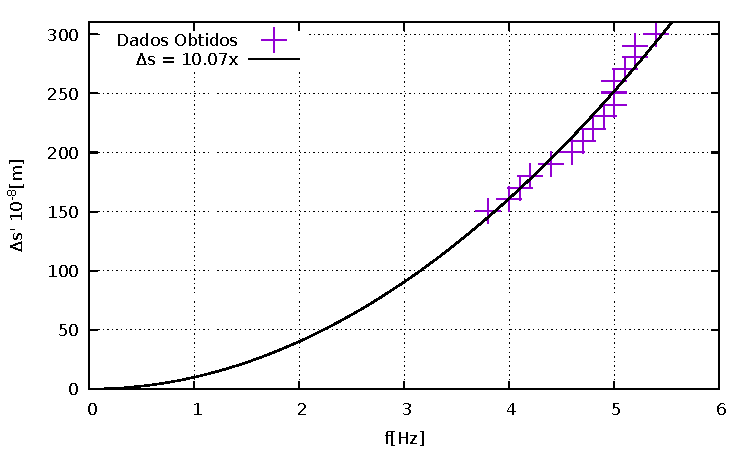
\includegraphics[scale= 1.0]{graf/e_m.pdf}
	\caption{Relação entre a diferença de potencial($DDP$) usado para acelerar os elétrons e o raio ($r$) formado pelos elétrons, com equação igual a $V = (98079.57\pm 1219.33)r^2$}
\label{fig}
\end{figure}

\subsection{Interpretação dos Resultados}

Sabendo-se que
\begin{equation}
	\frac{e}{m}=\frac{2V\left(\frac{5}{4}\right)^3a^2}{[N\mu _0 Ir]^2}
\end{equation}
é possível fazer
\begin{equation}
	V = \frac{[N \mu _0 I]^2\left(\frac{e}{m}\right)}{2(5/4)^3a^2}r^2
\end{equation}
onde fazendo
\begin{equation}
\begin{split}
	\lambda = \frac{[N \mu _0 I]^2\left(\frac{e}{m}\right)}{2(5/4)^3a^2}\\
	V = \lambda r^2
\label{eq1}
\end{split}
\end{equation}
sabendo que
\begin{equation}
	V = 98079,57r^2
\label{eq2}
\end{equation}
igualando \ref{eq1} e \ref{eq2} é obtido
\begin{equation*}
	\lambda = 98079,57
\end{equation*}
e portanto
\begin{equation}
	98079,57 =  \frac{[N \mu _0 I]^2\left(\frac{e}{m}\right)}{2(5/4)^3a^2}
\end{equation}
onde $N,\mu _0,I$ e $a$ são:
\begin{equation*}
	\begin{split}
		N=130\\
		\mu _0 =4\pi\times10^{-7}\\
		I=(1,24\pm0,01)A\\
		a=0,15cm
	\end{split}
\end{equation*}
substituindo os valores
\begin{equation}
	98079,57 =  \frac{[130*4\pi\times10^{-7}*1,24]^2\left(\frac{e}{m}\right)}{2(5/4)^30,15^2}
\end{equation}
e portanto
\begin{equation}
	\frac{e}{m}=\frac{98079,57*2*(5/4)^3*0,15^2}{[130*4\pi\times10^{-7}*124]^2}
\end{equation}
resolvendo
\begin{equation}
	\frac{e}{m}=(2,10\pm0,08)\times10^{11}Q/kg
\end{equation}
Comparando com o valor de 
\begin{equation}
	c=1,76\times10^{} Q/Kg
\end{equation}        
obtido na literatura \cite{PASCO}, resulta em um erro relativo ($Er$) de:
\begin{equation}
	Er=\left|\frac{1,76\times10^{11}-2,10\times10^{11}}{1,76\times10^{11}}\right|*100\%= 19,31\%
\end{equation}

Estes erros estão associados a obtenção dos dados, sendo
possível um erro de paralaxe durante a visualização dos dados na régua espelhada, o que acarreta uma variação do valor de $c$ predito na literatura. Porém, mesmo com todos os fatores associados, o erro  de
19,31\% é aceitável dentro da precisão necessária para a realização do experimento.

	
	\section{Conclusão}
Podemos dizer, com base no desvio obtido, que o experimento realizado foi bem sucedido. Mesmo com um erro pequeno, pode-se salientar alguns motivos pelo mesmo, como o movimento de pessoas no laboratório e a vibração do ar condicionado, visto que o aparelho é muito sensível, também, possíveis erros humanos na hora da contagem de franjas. Por fim, com o êxito do experimento, conseguimos determinar o índice de refração do ar satisfatoriamente. 

\vspace{3cm}
	\begin{thebibliography}{1}
    	\bibitem{PASCO}PASCO, \it{Interferometer}, Instruction Manual and Experiment Guide for the PASCO scientific Model 0S-8501.
	\end{thebibliography}	
	
\end{document}

